\documentclass[notheorems,xetex]{beamer}
%\documentclass[UTF8]{ctexbeamer}
\usepackage{xeCJK}%preamble part
%\usepackage{showframe}
\usepackage{amsmath, amsthm, amssymb}
\usepackage{graphicx}
\usepackage{bm}
\usepackage{caption}
\usepackage{ragged2e}
\usepackage{multirow}
\usepackage{float}
\usepackage{color}
%\usepackage[font=Helv,timeinterval=3]{tdclock}
\setbeamertemplate{theorems}[numbered]
\DeclareMathOperator*{\rgmax}{argmax}
\DeclareMathOperator*{\rgmin}{argmin}
\DeclareMathOperator{\tr}{tr}
%\setCJKmainfont{SimSun}[AutoFakeBold=false]
%\setsansfont{SimSun}
\setbeamertemplate{frametitle}[default][center]
\setbeamertemplate{footline}[frame number]
\setlength{\parindent}{0.8cm}
\theoremstyle{definition}
\newtheorem{theorem}{定理}
\newtheorem{lemma}{引理}
\newtheorem{definition}{定义}
\newtheorem{cor}{推论}
%\newcommand{\transpose}[1]{\ensuremath{#1^{\scriptscriptstyle T}}}
\usetheme{Warsaw}
%\usepackage{eforms}%设置倒计时
% eforms is windows only
%\begin{insDLJS}{showtime}{Show time}%embedding document level JavaScript, the first required variable is the base name, exports showtime.djs file.
%ttotal=30;%总时间自己设定, 分钟数
%stotal=ttotal*60
%function tClock()
%{%this.getField("datetime").value = util.printd("hh:MM:ss tt dd/mm/yyyy", new Date());
%stotal=stotal-1
%if (stotal>0) {    %%在stotal递减到0之前正常计算所剩时、分、秒
%hleft=Math.floor(stotal/3600)
%mleft=Math.floor((stotal - hleft*3600)/60)
%sleft=stotal - hleft*3600-mleft*60
%}
%else{    %%在stotal递减到0及负数时对所剩时、分、秒赋值0
%hleft=0
%mleft=0
%sleft=0
%}
%if (hleft>=1){this.getField("datetime").value=hleft+':'+mleft+':'+sleft;}
%else{this.getField("datetime").value=mleft+':'+sleft;}
%}
%var timeout =app.setInterval("tClock()",1000);
%\end{insDLJS}
%\newcommand{\timemark}%
%{\textField[\BC{0.2 0.2 0.7}\BG{0.2 0.2 0.7}%
% \textFont{TiRo}\textSize{5}\textColor{1 1 0 rg}]{datetime}{6mm}{1bp}}
%参数可以自己改
%\setbeamercovered{transparent}
%\usepackage{times}
\title{无线网络中定位信息的时空传播机理研究} % (optional, use only with long paper titles)
\author[赵丰]
{\quad \hbox to 9em{姓名: \hfil 赵丰}\\ \and \hbox to 9em{指导老师: \hfil 沈渊}\\ \and \hbox to 9em{联合指导老师: \hfil 梁恒}}
\institute[清华大学] % (optional, but mostly needed)
{\normalsize\quad
  清华大学数学科学系
}
\date{\the\year 年 \the\month 月 \the\day 日}
%\AtBeginSubsection[]
%{
%  \begin{frame}<beamer>{目录}
%    \tableofcontents[currentsection,currentsubsection]
%  \end{frame}
%}
\usefonttheme[onlymath]{serif}
\setbeamercolor{alerted text}{fg=blue}
\setbeamercolor{normal text}{bg=green!10!white}
\setbeamercolor{frametitle}{fg=blue!50!black,bg=white}
\begin{document}
\frame{\titlepage}
\date{\hspace{1mm} \timemark}
\begin{frame}{概要}
%\initclock
%\date{\the\year 年 \the\month 月 \the\day 日 {\Large\crono}}
  \tableofcontents
\end{frame}
\section{问题背景}%one frame only
%application case
\begin{frame}
协作定位技术有着广泛的应用前景:
  \begin{columns}[T] % contents are top vertically aligned
     \column{.5\textwidth}
     \begin{figure}
     \includegraphics[height=4cm]{UAV.jpg}
     \caption*{无人机编队}
     \end{figure}
     \column{.5\textwidth}
     \begin{figure}
     \includegraphics[height=4cm]{VL.jpg}
     \caption*{车联网}
     \end{figure}
     \end{columns}
\end{frame}
\section{数学模型}
%\subsection[非协作定位场景]{非协作定位场景}

%\subsection[协作定位场景]{协作定位场景}

%\begin{frame}{多个待测节点协作定位}
%考虑一个平面定位场景中不仅部署了$N_b$个位置已知的锚点,还有$N_a$个位置未知的待定位节点,某些位置未知的节点之间可以\alert{彼此测距},第i和第j个未知节点距离测量量服从均值为$||\bm{p}^a_i-\bm{p}^a_j||)$,方差为$\sigma_{ij}$的正态分布$X_{ij}$。
%
%以$N_a$个未知节点的位置$\{p_i^a\}$作为待估计的参数,可以得到测距量的联合概率密度函数为
%
%\begin{equation}
%\prod_{i=1}^{N_a} f(x^i_1,...x^{i}_{N_b}|\bm{p^a_i})\prod_{(i,j)\in \mathcal{E}}\frac{1}{\sqrt{2\pi\sigma^2}}exp(-\frac{(x_{ij}-f(||\bm{p}^a_i-\bm{p}^a_j||))^2}{2\sigma_{ij}^2})
%\end{equation}
%上式中$\mathcal{E}$表示可以彼此测距的未知节点的二元组的集合,而$x_t^i$表示第t个锚点和第i个未知节点的距离测量量。
%\end{frame}
%\begin{frame}{协作定位图示}
%        \begin{figure}
%          \centering
%          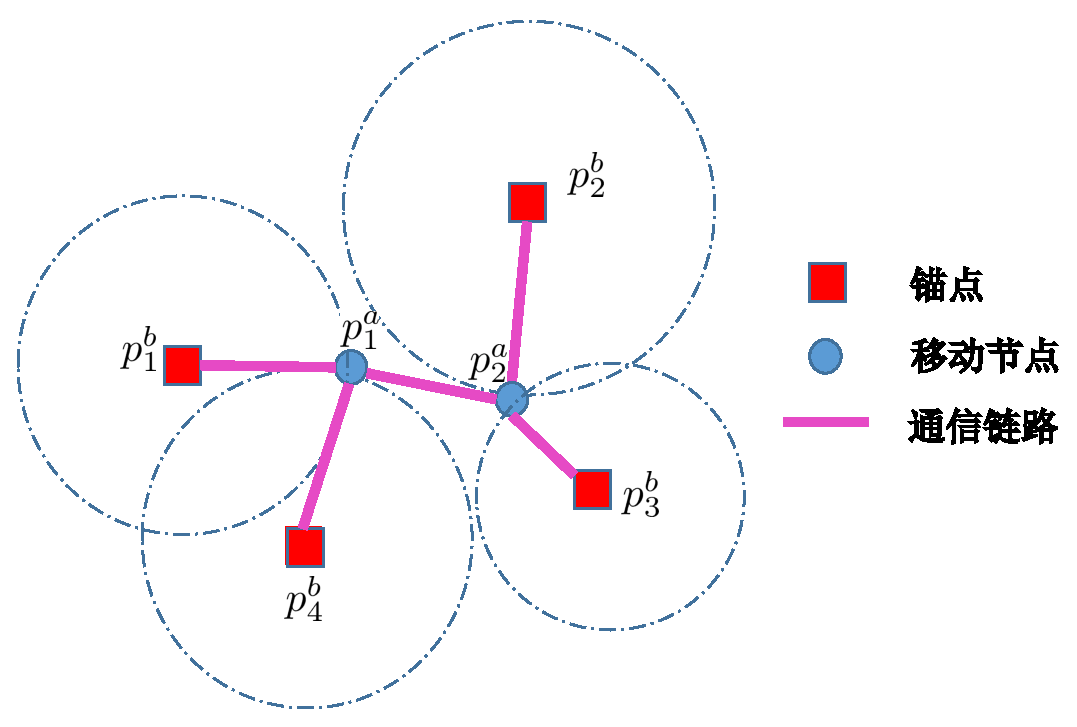
\includegraphics[width=300pt]{cooperative_spatial.eps}
%          \caption{协作静态场景下的定位}\label{fig:cooperative_spatial}
%        \end{figure}
%\end{frame}
%\begin{frame}{费舍尔信息矩阵}
%关于$2N_a$个参数$\{p_i^a\}$的费舍尔信息矩阵有如下的表达形式:
%\begin{equation}
%\scriptsize{
%I(\bm{P})=
%\left(
%\begin{array}{cccc}
%I_B(\bm{p}_1)+&-\bm{C}_{1,2}&...&-\bm{C}_{1,N_a}\\
%\sum_{j\in \{1,..N_a\}\backslash\{1\}}\bm{C}_{1,j}&&&\\
%&&&\\
%-\bm{C}_{1,2} & I_B(\bm{p}_2)+
%&...&-\bm{C}_{2,N_a}\\
%&\sum_{j\in \{1,..N_a\}\backslash \{2\}}\bm{C}_{2,j}&&\\
%&&&\\
%\vdots &\vdots&\ddots &\vdots\\
%&&&\\
%&&&I_B(\bm{p}_{N_a})+\\
%-\bm{C}_{1,N_a}&-\bm{C}_{2,N_a}&...& \sum_{j\in \{1,..N_a\}\backslash\{N_a\}}\bm{C}_{N_a,j}\\
%\end{array}
%\right)
%}
%\end{equation}
%上面的式子中$I_B(\bm{p}_i)$表示$N_b$个锚点对未知节点距离测量的贡献,和前面的(\ref{eq:uu})式相同。$C_{i,j}=\bm{1}_{(i,j)\in E}\lambda_{i,j}\bm{u}_{ij}\bm{u}_{ij}^{\textrm{T}}$,表示未知节点i和j协作的矩阵。
%$\bm{u}_{ij}=\frac{\bm{p}^a_i-\bm{p}^a_j}{||\bm{p}^a_i-\bm{p}^a_j||}$表示未知节点i和j的方向向量。
%\end{frame}
\subsection[空间协作定位]{空间协作定位}
\subsection[时间协作定位]{时间协作定位}
%\begin{frame}
%     单个节点在时间上的协作定位:
%     \begin{figure}
%          \centering
%          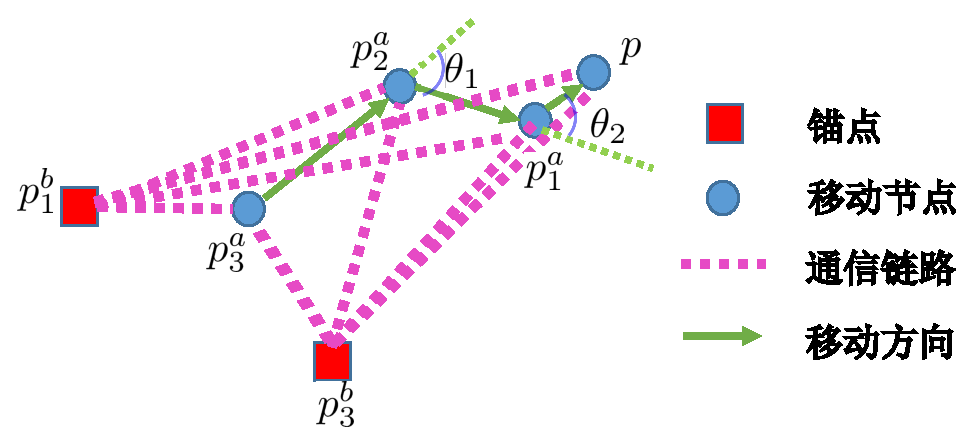
\includegraphics[height=4cm]{cooperative_single_temporal.eps}
%          \caption*{时间协作定位图示}
%     \end{figure}
%\end{frame}
\begin{frame}{数学模型}
\begin{itemize}
\item        场景中有$N_b$个位置已知的\alert{锚点}

\item        锚点在时刻$t_1,t_2,\dots,t_{N_a}$对待定位节点进行测距

\item        距离测量量服从正态分布

\item        节点在相邻时刻间可以测量速度,服从正态分布

\item        速度测量可以转化为节点相邻时刻间的距离测量
\end{itemize}
     \begin{figure}
          \centering
          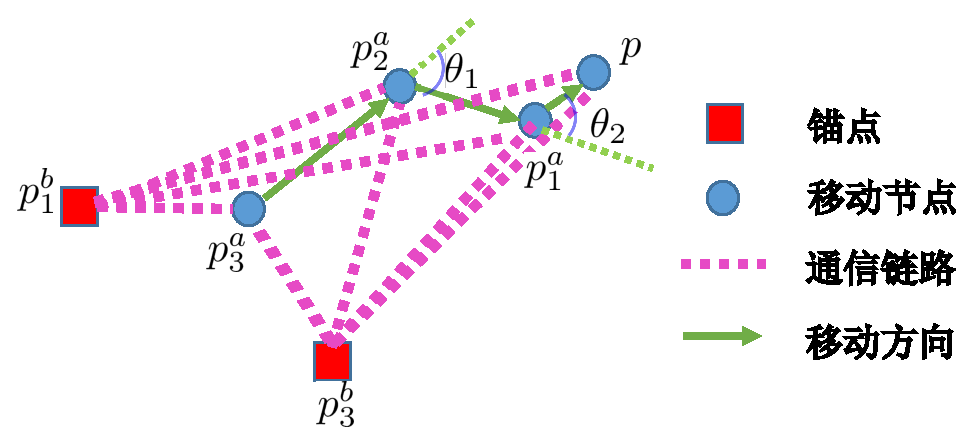
\includegraphics[height=4cm]{cooperative_single_temporal.eps}
          \caption*{时间协作定位图示}
     \end{figure}

\end{frame}
\begin{frame}
\begin{itemize}
\item 各个测量量彼此独立

\item 基于这些观测寻找对节点$\bm{p}$的位置估计最大可能的精度。

\pause
\item 根据点估计的理论,对于一个无偏估计量,它的方差的下界是\alert{费舍尔信息量}(Fisher Information)的倒数,称之为\alert{克拉美罗界}(Cram\'er-Rao Bound)。
\end{itemize}
     \begin{figure}
          \centering
          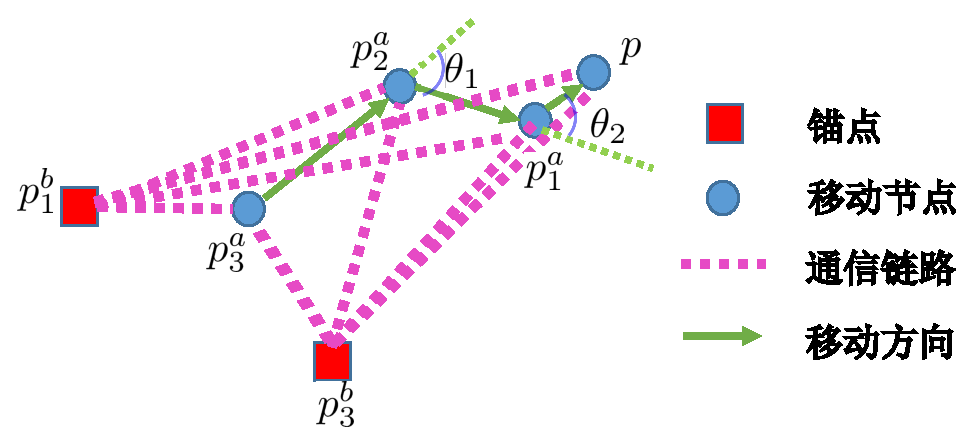
\includegraphics[height=4cm]{cooperative_single_temporal.eps}
     \end{figure}

\end{frame}
\begin{frame}
如果估计量是高维的(节点的\alert{2维}位置),费舍尔信息量推广为\alert{费舍尔信息矩阵}(Fisher Information Matrix)。


克拉美罗界在我们研究的问题中也称之为\alert{定位误差下界}(Spatial Position Error Bound),它的计算公式为:
\begin{equation*}
  \text{SPEB}=\text{tr}(\bm{I(\bm{p})}^{-1}).
\end{equation*}
     \begin{figure}
          \centering
          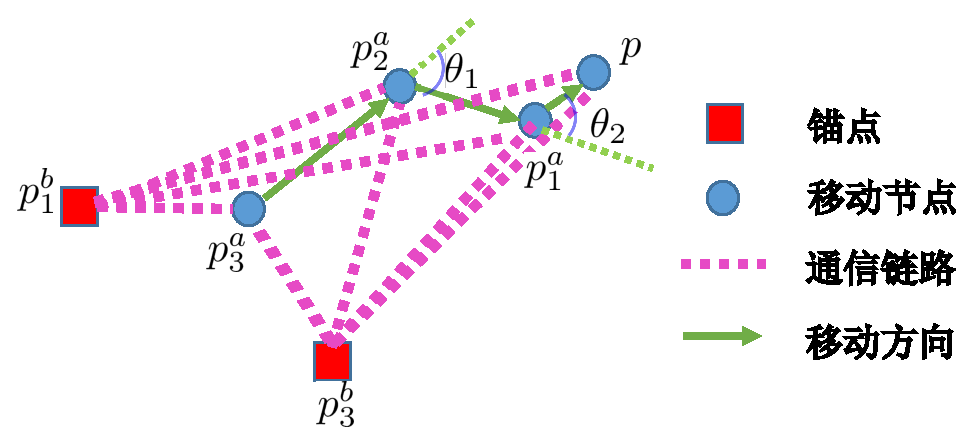
\includegraphics[height=4cm]{cooperative_single_temporal.eps}
     \end{figure}

%        \begin{figure}
%          \centering
%        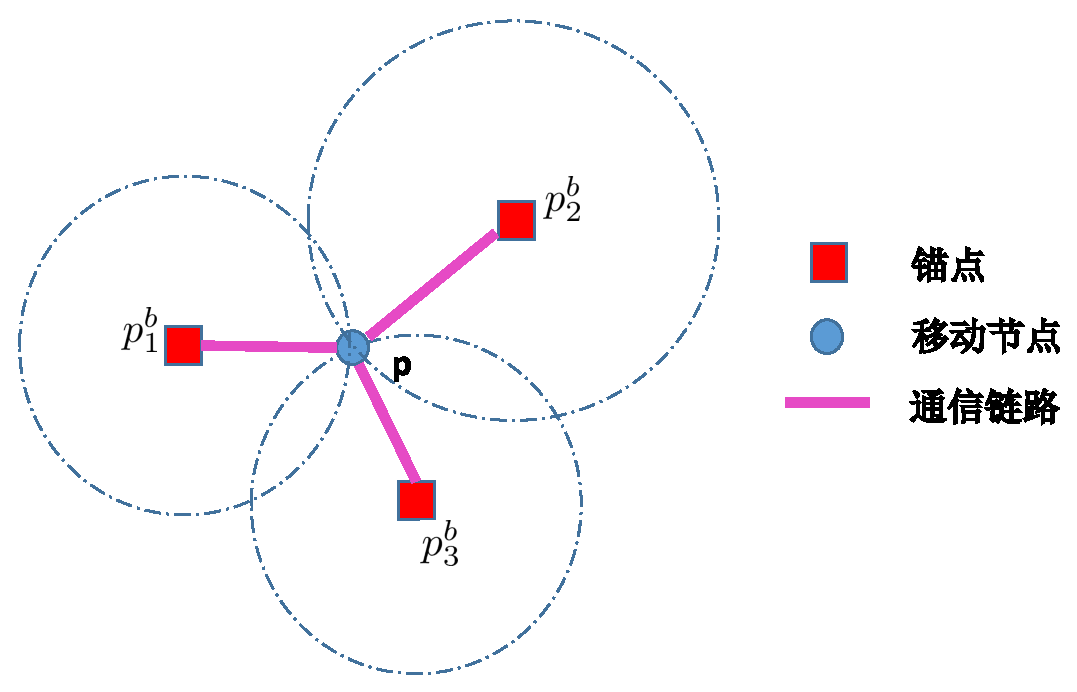
\includegraphics[width=250pt]{non_cooperative_spatial.eps}
%          \caption{非协作静态场景下的定位}\label{fig:non_cooperative_spatial}
%\end{figure}
\end{frame}

%\begin{frame}{费舍尔信息矩阵}
%以节点的\alert{2维}位置为待估计参数,费舍尔信息量推广为\alert{费舍尔信息矩阵}(Fisher Information Matrix)。
%
%对于我们的模型问题,费舍尔信息矩阵有如下的形式:
%\begin{equation}\label{eq:uu}
%I(\bm{p})=\displaystyle\sum_{i=1}^{N_b}\frac{1}{\sigma_i^2}\bm{u}_i\bm{u}_i^{\textrm{T}}
%\end{equation}
%其中
%\begin{equation}
%\bm{u_i}=\frac{\bm{p}^b_i-\bm{p}}{||\bm{p}^b_i-\bm{p}||}
%\end{equation}
%
%\end{frame}

%\begin{frame}
%假设测量时间间隔比较小使得相邻测量间节点速度方向可近似看作不变,速度测量值服从均值为$v$,方差为$\sigma_{v}$的正态分布$V_{ij}$。那么
%\end{frame}
\begin{frame}
以节点各时刻的的位置$\{p_i\}$作为待估计的参数,可以得到费舍尔信息矩阵有如下的表达形式


$\bm{I}(\bm{P})=$
\[
\begin{pmatrix}
a\bm{I}_2+&-b\bm{u}_1\bm{u}_1^{\textrm{T}}&\bm{0}&\dots&\bm{0}\\
+b\bm{u}_1\bm{u}_1^{\textrm{T}}&&&&\\
&&&&\\
-b\bm{u}_1\bm{u}_1^{\textrm{T}} & a\bm{I}_2+b\bm{u}_1\bm{u}_1^{\textrm{T}}&-b\bm{u}_2\bm{u}_2^{\textrm{T}}&\dots&\bm{0}\\
&+b\bm{u}_2\bm{u}_2^{\textrm{T}}&&&\\
\vdots &\vdots&\ddots &\vdots&\vdots\\
&&&&\\
\bm{0}&\bm{0}&...& -b\bm{u}_{N_a-1}\bm{u}_{N_a-1}^{\textrm{T}}&a\bm{I}_2+\\
&&&&+b\bm{u}_{N_a-1}\bm{u}_{N_a-1}^{\textrm{T}}\\
\end{pmatrix}.
\]
\pause
这里,费舍尔信息矩阵$\bm{I}(\bm{P})$具有块三对角的形式。
\end{frame}

%\section{简单网络}
%\subsection{非协作单节点定位网络}
%\begin{frame}{非协作单节点定位网络}
%一般的,对称正定的矩阵A定义了平面上椭圆方程$\bm{x}^{\textrm{T}}A\bm{x}=1$,
%对单节点定位误差的描述同样可以借助平面上的椭圆方程来描述:
%\begin{definition}
%对位置$\bm{p}$的2乘2的费舍尔信息矩阵$\bm{I}$定义了平面上的椭圆方程
%\begin{equation}\label{eq:ie}
%\bm{x}^{\textrm{T}}\,\bm{I}_{\bm{p}}^{-1}\bm{x}=1,\bm{x}\in \mathbb{R}^2.
%\end{equation}
%称之为节点位置的\alert{信息椭圆}。
%\end{definition}
%\pause
%信息椭圆各个主轴的长度衡量了特征值的大小,代表了该方向的定位精度。
%\end{frame}
%\begin{frame}
%对于非协作单节点定位场景,我们研究了信息椭圆离心率和定位误差下界的关系:
%\begin{figure}
%  \centering
%  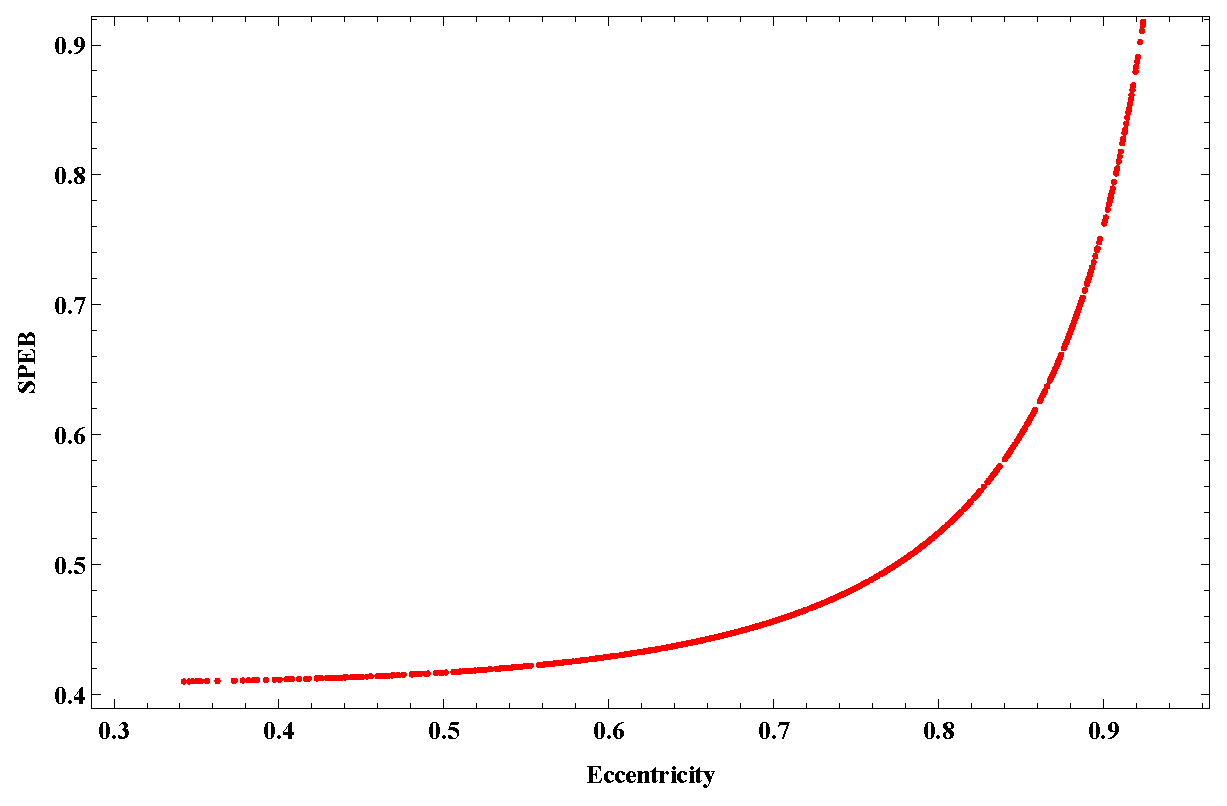
\includegraphics[width=300pt]{eccentricity_SPEB.eps}
%  \caption{定位误差下界与信息椭圆离心率的关系}\label{fig:eccentricity}
%\end{figure}
%\end{frame}
%\subsection{两个未知节点协作的场景}
%\begin{frame}
%两个移动节点协作情况下,我们可以借助下面的定理显示写出它们的位置的联合估计的费舍尔信息矩阵$I(\bm{P})$的特征多项式:
%\begin{theorem}\label{thm:ShenIden}
%设$J$是对称正定的矩阵,那么
%\begin{equation}\label{eq:ShenIden}
%|J+\epsilon \bm{u}\bm{u}^{\textrm{T}}|=|J|+\epsilon \bm{u}^{\textrm{T}}J^*\bm{u}
%\end{equation}
%其中$J^*$表示J的伴随矩阵,满足等式$JJ^*=|J|\bm{I}$
%\end{theorem}
%\pause
%借助上面的定理可以求
%\begin{equation}
%I(\bm{P})=\left(\begin{array}{cc}
%\bm{\Sigma}_0+\epsilon \bm{u}\bm{u}^{\textrm{T}}  &-\epsilon \bm{u}\bm{u}^{\textrm{T}}  \\
%-\epsilon \bm{u}\bm{u}^{\textrm{T}}  & \bm{\Sigma}_1+\epsilon \bm{u}\bm{u}^{\textrm{T}}
%\end{array}
%\right).
%\end{equation}
%的特征值。
%\end{frame}
%\section{特殊结构网络}
%\subsection{特殊的全连接网络}
%\begin{frame}{全连接网络描述与求解}
%在协作定位网络的问题模型下,给出一些简化条件后考虑$2N_a$维的联合位置估计的费舍尔信息矩阵具有如下形式:
%$I(\bm{P})=a\bm{I}_{2N}+b\bm{J}$,
%  \begin{columns}[T] % contents are top vertically aligned
%     \begin{column}[T]{5cm}
%     其中
%\[
%\bm{J}_{ij}=\begin{cases}
%\sum_{k=1,k\neq i}^N \bm{u}_{ik}\bm{u}_{ik}^{\textrm{T}}&i=j\\
%-\bm{u}_{ij}\bm{u}_{ij}^{\textrm{T}}&i\neq j
%\end{cases}
%\]
%   比如对$N=5$的情形,有$\bm{u}_{12}=\left(\cos(\frac{2\pi}{5}),\sin(\frac{2\pi}{5})\right)$
%     \end{column}
%     \begin{column}[T]{5cm}
%          \includegraphics[height=4cm]{pentagon.eps}
%     \end{column}
%     \end{columns}
%
%
%\end{frame}
%\begin{frame}
%关于矩阵$\bm{I}(\bm{P})$瑞利商为:
%\begin{equation}
%R(\bm{x})=b\sum_{i\leq j\leq N} (\bm{u}_{ij}^{\textrm{T}}(\bm{x}_i-\bm{x}_j))^2+a,\bm{x}_i\in \mathbb{R}^2
%\end{equation}
%其中$\bm{x}=(\bm{x}_1,\bm{x}_2,\dots,\bm{x}_N) \in \mathbb{R}^{2N}$且$||\bm{x}||=1$
%\pause
%
%
%容易看出,当$\bm{x}_i=\bm{x}_j$或$(\bm{x}_i-\bm{x}_j)$与$\bm{u}_{ij}$正交时,瑞利商$R(\bm{x})$取到最小值a,
%进一步可证明$I(\bm{P})$的最大特征值是$a+Nb$,且其余的特征值均为$a+Nb/2$
%\end{frame}
\section{线型网络}
\subsection{直接法}
\begin{frame}{直接法}
直接法可以给出当节点作直线运动时的平均定位误差下界:
\begin{align*}
  \text{SPEB}=&\lim_{N_a \to \infty}\frac{\tr(\bm{I(\bm{P})}^{-1})}{N_a}\\
  =&\frac{1}{a}+\frac{1}{\sqrt{a^2+4ab}}\\
\end{align*}
{\noindent 方法简述:}

$a$是$\bm{I}(\bm{P})$的$ n+1$重特征值,其余$n-1$个特征值为
\[
a+2b\left(1-\cos\frac{\pi j}{n}\right),j=1,\dots,n-1
\]
\end{frame}
%我们可以用直接法给出节点作直线运动时的平均定位误差下界:
%\pause
\begin{frame}
%$\bm{K}_{n-1}=2\bm{I}_{n-1}-\bm{S}$,由引理(\ref{lemma:special})可求出$\bm{K}_{n-1}$的全部特征值。
%\pause
\[
f(n):=\frac{\tr(\bm{I}(\bm{P})^{-1})}{n}=\frac{1}{n}\left(\frac{n+1}{a}+\sum_{j=1}^{n-1}\frac{1}{a+2b(1-\cos(\frac{\pi j}{n}))}\right)
\]
当$n\to \infty$,根据Riemann积分的定义:
\[
\lim_{n\rightarrow \infty}f(n)=\frac{1}{a}+\int_0^1 \frac{1}{a+2b(1-\cos(\pi x))}dx
\]
化为复积分由留数定理可得
\[
\lim_{n\rightarrow \infty}f(n)=\frac{1}{a}+\frac{1}{\sqrt{a^2+4ab}}.
\]
\end{frame}
\begin{frame}
$a$和${\sqrt{a^2+4ab}}$分别代表了平均定位误差下界在两个方向的信息量。


一般的,对平面上节点的位置估计的精度可以借助平面上的椭圆方程来描述:
\begin{definition}
关于位置$\bm{p}$的$2\times 2$的费舍尔信息矩阵$\bm{I}$定义了平面上的椭圆方程
\[
\bm{x}^{\textrm{T}}\,\bm{I}_{\bm{p}}^{-1}\bm{x}=1,\bm{x}\in \mathbb{R}^2.
\]
称之为节点位置$\bm{p}$的\alert{信息椭圆}。
\end{definition}
\pause
\end{frame}
\begin{frame}
信息椭圆各个主轴的长度衡量了特征值的大小,代表了该方向的定位精度。

采样时刻$N_a$很大,协作强度$b=1$,锚点定位强度$a=\lambda$:
%\the\hsize\par
%\the\vsize\par
%\the\textwidth\par
%\the\linewidth
\begin{figure}
\centering
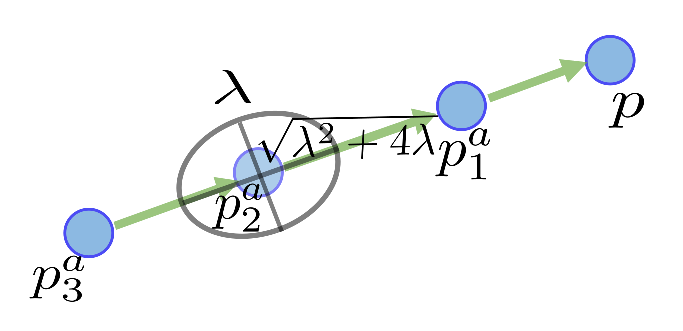
\includegraphics[width=0.8\textwidth]{direct.eps}
\caption*{信息椭圆图示}
\end{figure}
\end{frame}
%\begin{frame}{用等效费舍尔信息矩阵求解节点平均定位误差}
%给定两组数列$\{a_n\}$和$\{b_n\}$我们可以构造
%\[
%x_n=a_0+\cfrac{b_1}{a_1+\cfrac{b_2}{a_2+\dots+\cfrac{b_n}{a_n}}},\scriptsize{J=\left(
%\begin{array}{ccccccc}
%2K_1&-K_1&-K_1&0&\dots&&\\
%-K_1&2K_1&0&-K_1&0\dots&\\
%-K_1&0&2K_1&0&-K_1&0&\dots\\
%0&-K_1&0&2K_1&0&\dots&\\
%\vdots&\vdots&&\ddots&\dots&\\
%\end{array}
%\right)}
%\]
%右边的J是对节点重排后的结果,将线性网络中心的节点放到了矩阵的左上角,求解该问题还需要如下定理:
%\begin{theorem}[fundamental recurrence formulas]
%设$x_n=\frac{h_n}{k_n}$,则有如下递推关系成立:
%\vspace{-3mm}
%\begin{eqnarray}
%h_n=a_nh_{n-1}+b_nh_{n-2}\\
%k_n=a_nk_{n-1}+b_nk_{n-2}
%\end{eqnarray}
%\end{theorem}
%\end{frame}
%\begin{frame}
%为简化计算,对$a\bm{I}+b\bm{J}$提取b,记$\lambda=\frac{a}{b}$
%通过等效费舍尔信息矩阵的公式可以推导出关于矩阵$(\lambda\bm{I}+\bm{J})$左上角的2乘2矩阵的等效费舍尔信息矩阵实际是个对角阵,其中一个对角元为$\lambda$,另一个对角元为可以写成如下连分式的形式:
%\[
%\lambda+2-\cfrac{2}{\lambda+2-\cfrac{1}{\lambda+2-\cfrac{1}{\lambda+2-\dots}}}
%\]
%使用上页的定理,解常系数差分方程得通解为$\frac{h_n}{k_n}=\frac{A_1x_1^n+B_1x_2^n}{A_2x_1^n+B_2x_2^n}$
%递推公式的初始条件是
%\vspace{-2mm}
%\[
%h_0=\lambda+2,k_0=1,h_1=\lambda+2-\frac{2}{\lambda+2},k_1=\lambda+2
%\]
%其中$x_{1,2}=\frac{\lambda+2\pm \sqrt{\lambda^2+4\lambda}}{2}$
%由于$|\frac{x_1}{x_2}|>1$,所以极限$\lim_{n\to \infty}\frac{h_n}{k_n}=\frac{A_1}{A_2}$
%$A_1,A_2$可由初始条件求出,它们的比值是$\sqrt{\lambda^2+4\lambda}$
%\end{frame}
%


\subsection{连分式法}
\begin{frame}{连分式法}
     终点$p$的信息椭圆在只有锚点定位的情况下是一个圆。

%  \begin{columns}[T] % contents are top vertically aligned
 %    \begin{column}[T]{7cm}
     \begin{equation*}
    T_1=\lambda
     \end{equation*}
  %    \end{column}
   %  \begin{column}[T]{3cm} % alternative top-align that's better for graphics
        \begin{figure}
          \centering
          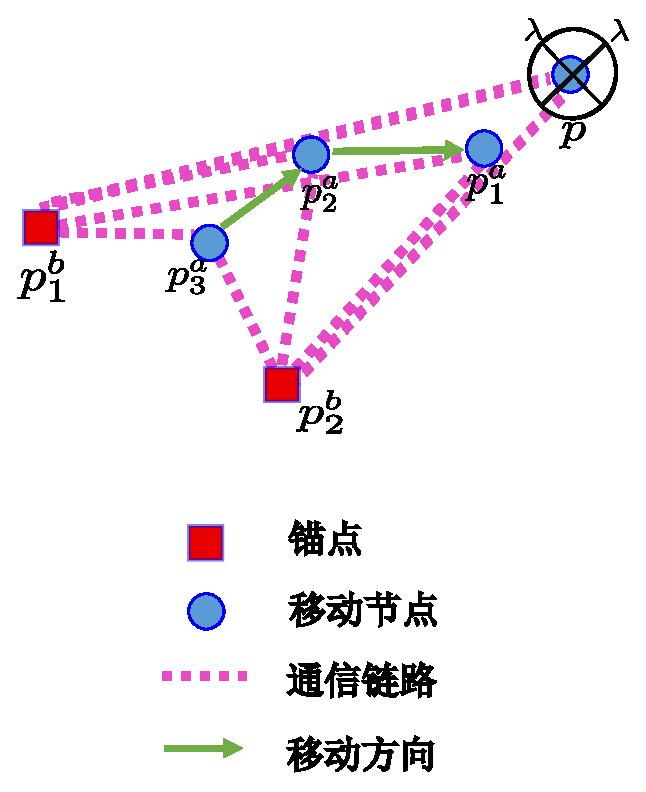
\includegraphics[width=120pt]{direct_single_temporal_pre.eps}
        \end{figure}
    % \end{column}
    % \end{columns}
  \end{frame}
  \begin{frame}
     增加了和上一时刻的协作链路后终点$p$的信息椭圆在沿$\bm{p}\bm{p}_1^a$方向上的信息$T_1$可以写成连分式的形式:
     \begin{equation*}
T_1=\lambda+\cfrac{1}{1+\cfrac{\sin^2 \theta_1}{\lambda}+\cfrac{\cos^2\theta_1}{\lambda+\cfrac{1}{1+\cfrac{\sin^2 \theta_2}{\lambda}+\cfrac{\cos^2\theta_2}{\lambda+\boxed{\cfrac{1}{1+\cfrac{1}{\lambda}}}}}}}.
     \end{equation*}
%\raggedright{
%\fbox{\includegraphics[width=160pt]{../presentation/direct_single_normal.eps}}
%}
%\vskip -9em
%\parbox[c][6em][t]{0.33\textwidth}{距$\bm{p}$较远的节点$\bm{p}_3^a$提供的信息在连分式的最内侧}
\begin{tabular}{lr}
\multirow[t]{4}{*}[-3em]{\fbox{\includegraphics[width=160pt]{direct_single_normal.eps}}}&\parbox[c][6em][t]{0.33\textwidth}{距$\bm{p}$较远的节点$\bm{p}_3^a$提供的信息在连分式的最内侧}\\
\end{tabular}
%\fbox{\includegraphics[width=160pt]{../presentation/direct_single_normal.eps}}
  \end{frame}

    \begin{frame}
     考虑增加一个角度参数$\theta_{N_a}$,由此得到的新的$T_1$记为$T'_1(N_a)$,研究$T'_1(N_a)$比原来的$T_1(N_a)$增大的量。
%  \begin{columns}[T] % contents are top vertically aligned
 %    \begin{column}[T]{7cm}
 \begin{equation*}
T'_1=\lambda+\cfrac{1}{1+\cfrac{\sin^2 \theta_1}{\lambda}+\cfrac{\cos^2\theta_1}{\dots+\cfrac{\dots}{1+\cfrac{\sin^2 \theta_3}{\lambda}+\cfrac{\cos^2\theta_3}{\lambda+\cfrac{1}{1+\cfrac{1}{\lambda}}}
}}}.
     \end{equation*}
%     \vskip -6em
  %   \end{column}
   %  \begin{column}[T]{3cm} % alternative top-align that's better for graphics
 \raggedright{
\fbox{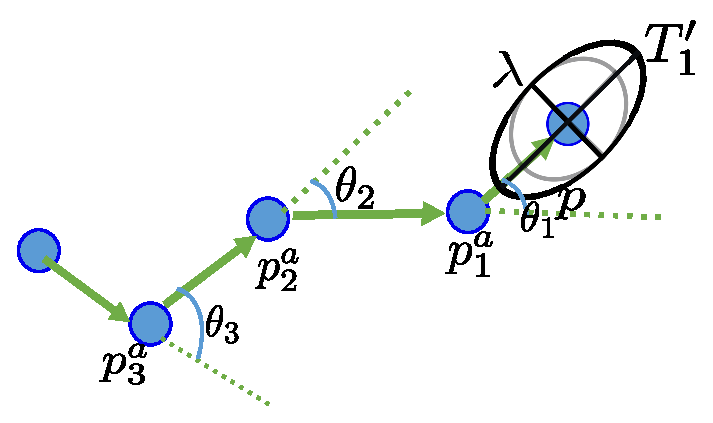
\includegraphics[width=160pt]{direct_single_normal_after.eps}}
}
%\vskip -6em

%         \quad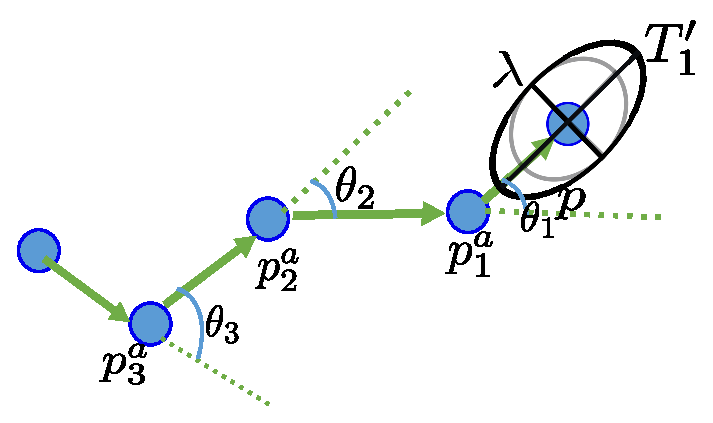
\includegraphics[width=120pt]{direct_single_normal_after.eps}
    % \end{column}
     %\end{columns}
  \end{frame}
\begin{frame}
一般地,可以得到终点时刻信息椭圆短轴方向的特征值为$\lambda$,长轴方向的特征值$T_1$可以用连分式表示。

设$\bm{u}_i=(\cos\theta_i,\sin\theta_i)^{\textrm{T}}$
\begin{equation*}
\begin{split}
T_{i-1} =& \lambda + \frac{1}{1+\frac{\sin^2\theta_i}{\lambda}+\frac{\cos^2\theta_i}{T_i}},2\leq i\leq N_a-1\\
T_{N_a-1}  =& \lambda+\frac{1}{1+1/\lambda}
\end{split}
\end{equation*}

%$T_1$就是$U_{N_a}$的另一个特征值。
\pause
记增量$\Delta_+ T_1(N_a):=T'_1(N_a)-T_1(N_a)$,则我们可以得到
%$N_a=1$时有$\Delta_{+} T_{1}=\frac{\lambda}{\lambda+1}$,
$N_a\geq 2$时$\Delta_+ T_1(N_a)$满足:
\begin{equation*}
%\begin{split}
%\frac{(\cos\Delta\theta)^{2(N_a-1)}}{(1+1/\lambda)^2(\lambda^2+2\lambda)(2+\lambda)^{2(N_a-2)}}\leq & \Delta_+ T_1(N_a)\\
\Delta_+ T_1(N_a)\leq \frac{1}{(\lambda^2+2\lambda)(1+\lambda)^{2(N_a-2)}}.
%\end{split}
\end{equation*}
从而得到$N_a\to \infty$时$T_1$的收敛性。
%$T_1$是关于$\theta_1,\dots,\theta_{N_a-1}$的减函数,关于$N_a$的增函数。
\end{frame}
\begin{frame}
基于连分式法,取$\theta_i \sim U[0,2\pi]$的随机数,增量$T_1'(N_a)-T_1(N_a)$随$N_a$变化的仿真结果如下图所示
\begin{figure}
  \centering
  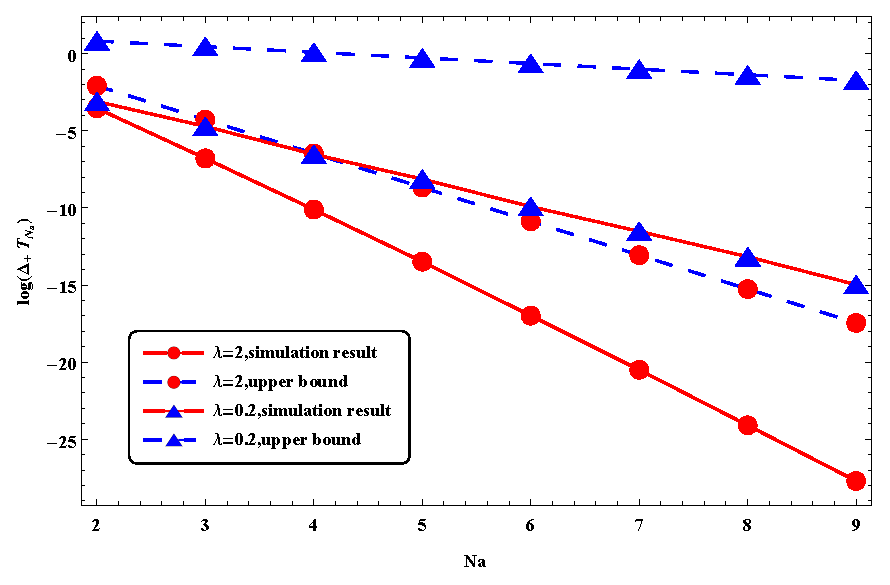
\includegraphics[width=280pt]{decreasing_exponential.eps}
  \caption*{协作链路信息衰减图示}\label{fig:continuous_fraction_exponential}
\end{figure}
\end{frame}
\begin{frame}
\begin{columns}[c]
 \begin{column}{.5\textwidth} % column designated by a command
 \begin{block}{衰减规律}
$N_a$条链路之外增加一层协作链路使目标节点定位误差的下降的数量是随$N_a$\alert{指数衰减}的。
\end{block}
\begin{block}{工程启示}
对某时刻的节点进行定位时,只需考虑其前后几个时刻的位置即可,较远的时刻基本没有信息量。
\end{block}
\end{column}
    \begin{column}{.5\textwidth}
       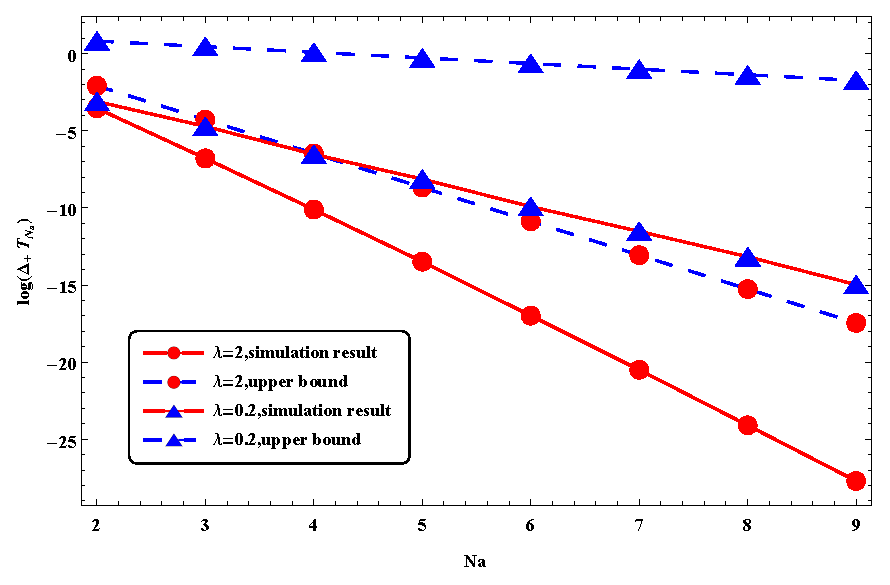
\includegraphics[width=160pt]{decreasing_exponential.eps}
       \end{column}
    \end{columns}
%为说明此结论,使用下面的记号
%\[
%[t_1,t_2,\dots,t_{n-1},t_n]=t_1+\cfrac{1}{t_2+\cfrac{1}{t_3+\dots+\cfrac{1}{t_{n-1}+\cfrac{1}{t_n}}}}
%\]
\end{frame}
%\begin{frame}{连分式的基本知识}
%\framesubtitle{有理数的有限连分式展开}
%\[
%\frac{682}{305}=2+\frac{72}{305}+2+\frac{1}{305/72}=2+\cfrac{1}{4+\cfrac{17}{72}}=\dots=2+\cfrac{1}{4+\cfrac{1}{4+\cfrac{1}{4+1/4}}}
%\]
%\end{frame}
%\begin{frame}
%\begin{itemize}
%  \item {欧几里得辗转相除法
%                \begin{eqnarray*}
%                 % \nonumber % Remove numbering (before each equation)
%                   682 =305\times2+72 & q_0=2\\
%                   305 = 72\times4+17 & q_1=4\\
%                   \dots = \dots& \\
%                   4 = 1\times4 &q_n=4
%                 \end{eqnarray*}
%                 }
%  \item {一个有理数表示为分数,一个分数看成两个整数的除法,可以用欧几里得法分解得出一系列的商$q_i$,
%  \[
%  \frac{682}{305}=q_0+\cfrac{1}{q_1+\cfrac{1}{q_2+\dots+1/q_n}}
%  \]
%  }
%\end{itemize}
%\end{frame}
%\begin{frame}{无理数的连分式展开}
%\begin{eqnarray*}
%\sqrt{5}=2+x_0&0<x_0<1\\
%\frac{1}{x_0}=4+x_1&0<x_1<1\\
%\dots&\dots\\
%\frac{1}{x_{n-1}}=4+x_n&0<x_n<1
%\end{eqnarray*}
%\[
%\sqrt{5}=2+\cfrac{1}{4+\cfrac{1}{4+\cfrac{1}{4+\dots}}}
%\]
%\end{frame}
%\begin{frame}
%记增量$\Delta_+ T_1(N_a):=T'_1(N_a)-T_1(N_a)$,则我们有如下结论:
%$N_a=1$时有$\Delta_{+} T_{1}=\frac{\lambda}{\lambda+1}$,
%
%$N_a\geq 2$时$\Delta_+ T_1(N_a)$满足:
%\begin{equation*}
%\begin{split}
%\frac{(\cos\Delta\theta)^{2(N_a-1)}}{(1+1/\lambda)^2(\lambda^2+2\lambda)(2+\lambda)^{2(N_a-2)}}\leq & \Delta_+ T_1(N_a)\\
%\Delta_+ T_1(N_a)\leq & \frac{1}{(\lambda^2+2\lambda)(1+\lambda)^{2(N_a-2)}}.
%\end{split}
%\end{equation*}
%\pause
%
%上式中
%\[
%\Delta \theta=\max_{2\leq k \leq N_a-1}|\theta_k|,\theta_k\leq \frac{\pi}{2}
%\]
%\end{frame}
\begin{frame}
$T_1$是关于$\theta_1,\dots,\theta_{N_a-1}$的减函数,关于$N_a$的增函数。

$T_1$方向上的信息量有一个上界,当诸夹角均趋于0且时间协作数量$N_a\to \infty$,这个上界可以达到:
\begin{equation*}
\lim_{\Delta \theta\to 0,N_a\to \infty}T_1(N_a)=\frac{\lambda+\sqrt{\lambda^2+4\lambda}}{2}
\end{equation*}
其中
\[
\Delta \theta=\max_{2\leq k \leq N_a-1}|\theta_k|
\]

%因为如果某个$\theta_i$等于90度,那么有限连分式$T_1$中就在$\theta_i$处截断了。
\end{frame}



%\begin{definition}
%  序列$t_1,t_2,\dots,t_r$;对于$j\geq2$可以递推地定义有限连分式$[t_1,t_2,\dots,t_r]:=t_1+\frac{1}{[t_2,\dots,t_r]}$
%\end{definition}
%比如
%\begin{align*}
%[2,4,4,4,4]&=2+\frac{1}{[4,4,4,4]}\\
%&=2+\frac{1}{4+\frac{1}{[4,4,4]}}
%\end{align*}
%一个有限连分式从定义上来说是从后往前算的,下面的定理指出可以从前往后算:
%\end{frame}
%\begin{frame}
%\begin{theorem}\label{thm:basic}
%设$a_{-1}=0,b_{-1}=1;a_0=1,b_0=0;$\\
%$a_n=t_n a_{n-1}+a_{n-2},b_n=t_n b_{n-1}+b_{n-2};n\geq 1$
%那么
%\begin{align*}
%[t_1,t_2,\dots,t_n]&=\frac{a_n}{b_n}\\
%&=\frac{t_n a_{n-1}+a_{n-2}}{t_n b_{n-1}+b_{n-2}}
%\end{align*}
%  设$p_j=t_j p_{j-1}+p_{j-2},q_j=t_j q_{j-1}+q_{j-2}$,$M_j=(\begin{matrix}p_j&q_j\\p_{j-1}&q_{j-1}\end{matrix})$
%  $p_0,p_1,q_0,q_1$由$M_0=I_2$给出,$T_j=(\begin{matrix}t_j&1\\1&0\end{matrix})$
%  则$M_j=T_jM_{j-1}$,递推得到$\binom{p_j}{q_j}=(\prod_{i=1}^r T_i )\binom{1}{0}$且
%  $[t_1,t_2,\dots,t_r]=\frac{p_r}{q_r}$
%\end{theorem}
%比如为计算$[2,4,4,4,4]\approx 2.236$
%\begin{tabular}{lll}
%  % after \\: \hline or \cline{col1-col2} \cline{col3-col4} ...
%  $a_1=2a_0+a_{-1}=2$ & $b_1=2b_0+b_{-1}=1$ &$[2]=\frac{a_1}{b_1}=2$ \\
%  $a_2=4a_1+a_0=9$ & $b_2=4b_1+b_0=4$ & $[2,4]=\frac{a_2}{b_2}=2.25$\\
%  $a_3=4a_2+a_1=38$ & $b_3=4b_2+b_1=17$ & $[2,4,4]=\frac{a_3}{b_3}=2.235$\\
%  \dots &\dots &\dots
%\end{tabular}
%\end{frame}
%\begin{frame}
%关于定理\ref{thm:basic}的理解:
%化简后是关于z的分式线性变换:
%\[
%[t_1,t_2,\dots,t_{n-1},z]=\frac{az+a'}{bz+b'}
%\]
%考虑$z\to \infty$得$[t_1,t_2,\dots,t_{n-1},z]\to[t_1,t_2,\dots,t_{n-1}]$
%\[
%\Longrightarrow \frac{a}{b}=\frac{a_{n-1}}{b_{n-1}}
%\]
%\end{frame}
%\begin{frame}
%\[
%[t_1,t_2,\dots,t_{n-1},z]=\frac{az+a'}{bz+b'}
%\]
%考虑$z\to 0$得$[t_1,t_2,\dots,t_{n-1},z]\to[t_1,t_2,\dots,t_{n-2}]$
%\[
%\Longrightarrow \frac{a'}{b'}=\frac{a_{n-2}}{b_{n-2}}
%\]
%\end{frame}
%\begin{frame}
%\begin{align*}
%  [t_1,t_2,\dots,t_{n-1},z]&=\frac{az+a'}{bz+b'}\\
% \frac{a}{b}&=\frac{a_{n-1}}{b_{n-1}}\\
% \frac{a'}{b'}&=\frac{a_{n-2}}{b_{n-2}}
%\end{align*}
%严格来说
%\begin{align*}
%  [t_1,t_2,\dots,t_{n-1},z]&=[t_1,t_2,\dots,t_{n-2},t_{n-1}+\frac{1}{z}]\\
%  &=\frac{(t_{n-1}+\frac{1}{z})a_{n-2}+a_{n-3}}{(t_{n-1}+\frac{1}{z})b_{n-2}+b_{n-3}}\\
%  &=\frac{a_{n-1}+\frac{1}{z}a_{n-2}}{b_{n-1}+\frac{1}{z}b_{n-2}}
%\end{align*}
%\end{frame}
%\begin{frame}
%\begin{theorem}
%$\lim_{r\to \infty}[t_1,t_2,\dots,t_r]$存在,且极限是形如$\frac{a+b\sqrt{m}}{c}$的二次根式当且仅当序列$t_2,t_3,\dots,$是循%环的。设$(\begin{matrix}a&b\\c&d\end{matrix})=(\prod_{i=1}^{rc} T_i)$,rc是循环周期,则极限x满足二次方程$x=\frac{ax+b}%{cx+d}$
%\end{theorem}
%可以用$[2,4,4,4,\dots]$表示数列$\{[2],[2,4],[2,4,4],\dots\}$的极限?
%这个极限为什么是$\sqrt{5}$?
%\[
%[4,4,4,\dots]=4+\frac{1}{[4,4,4,\dots]}
%\]
%设$x=[4,4,4,\dots]$,解方程得正根$x=2+\sqrt{5}$
%\begin{align*}
%[2,4,4,\dots]&=2+\frac{1}{[4,4,4,\dots]}\\
%&=\sqrt{5}
%\end{align*}
%\end{frame}
%\begin{frame}
%数列$\{[2],[2,4],[2,4,4],\dots\}$收敛到$\sqrt{5}$的速度有多快?
%\begin{align*}
%|[t_1,t_2,\dots,t_n]-[t_1,t_2,\dots,t_{n-1}]|&=\frac{t_n a_{n-1}+a_{n-2}}{t_n b_{n-1}+b_{n-2}}-\frac{a_{n-1}}{b_{n-1}}\\
%&=\frac{a_{n-2}b_{n-1}-a_{n-1}b_{n-2}}{b_n b_{n-1}}\\
%&=-\frac{a_{n-3}b_{n-2}-a_{n-2}b_{n-3}}{b_n b_{n-1}}\\
%&=\frac{(-1)^n}{b_n b_{n-1}}
%\end{align*}
%注意到:
%\begin{align*}
%b_n=&4 b_{n-1}+b_{n-2},n\geq 2;b_0=0,b_1=1\\
%\Longrightarrow & b_n \sim \frac{(2+\sqrt{5})^n}{2\sqrt{5}}
%\end{align*}
%推广基本连分式得到下面关于拓展连分式的定义:
%\begin{definition}
%  两组有限序列$\{a_1,\dots,a_r\},\{b_1,\dots,b_r\}$递推地定义数列$\{x_1,\dots,x_r\}$,%$x_0=\frac{a_r}{b_r},x_i:=a_{r-i}+\frac{b_{r-i}}{x_{i-1}},1\leq i\leq r-1$
%\end{definition}
%上面是一种后向求算的方法,类比基本连分式有前向递推公式,这里取$T_j=(\begin{matrix}a_j&b_j\\1&0\end{matrix})$即%有(\ref{thm:basic})
%的结果,并且由这个递推公式可以用归纳法证明欧拉连分式定理:
%\end{frame}
%\begin{frame}
%所以
%\begin{align*}
%|[2,4,4,4,\dots]-[2,\underbrace{4,4,\dots,4}_{\text{n-item}}]|\leq& \frac{1}{2\sqrt{5}}\sum_{i=n}^{\infty}\frac{1}{(2+\sqrt{5})^{2n+1}}\\
%  =& \frac{c}{(2+\sqrt{5})^{2n}}
%\end{align*}
%
%和牛顿迭代法
%\[
%x_{n+1}=\frac{1}{2}(x_n+\frac{5}{x_n})
%\]
%\quad 相比如何?
%\begin{align*}
%|x_{n+1}-\sqrt{5}|= & \frac{(x_n-\sqrt{5})^2}{2x_n},x_n\geq 2\\
%\leq &\left(\frac{x_0-\sqrt{5}}{2}\right)^{2n}
%\end{align*}
%\end{frame}
%牛顿迭代法和连分式都是指数收敛的。
%\pause
%如何理解连分式是指数收敛的?
%考虑连分式
%\begin{align*}
%\frac{\lambda+\sqrt{4\lambda+\lambda^2}}{2}=&\lambda+\cfrac{1}{1+\cfrac{1}{\lambda+\cfrac{1}{1+\cfrac{1}{\lambda+\dots}}}}\\
%=&[\lambda,1,\lambda,1,\dots].
%\end{align*}
%通过求解方程
%\[
%x=\lambda+\cfrac{1}{1+\cfrac{1}{x}}
%\]
%可以形式地得到连分式序列$\{[\lambda,1],[\lambda,1,\lambda,1],\dots,\}$的不动点
%\[
%x=\frac{\lambda+\sqrt{4\lambda+\lambda^2}}{2}
%\]
%\end{frame}
%\begin{frame}
%下面我们考虑由任意给定的角度序列$[\theta_2,\theta_2,\dots,\theta_{N_a-1}]$和正数$\lambda$ 构成的的有限连分式序列:
%\begin{equation*}\label{eq:recursive_efim}
%\begin{split}
%\underbrace{T_{i-1}-\lambda}_{M} & =\frac{1}{1+\frac{\sin^2\theta_i}{\lambda}+\frac{\cos^2\theta_i}{T_i}},2\leq i\leq N_a-1\\
%T_{N_a-1} & = \lambda+\frac{1}{1+1/\lambda}
%\end{split}
%\end{equation*}
%\pause
%如果我们考虑增加一个角度参数$\theta_{N_a}$,由此得到的新的$T_1$记为$T'_1(N_a)$,那么$T'_1(N_a)$比原来的$T_1(N_a)$增大了多少?
%$[t_1,t_2,\dots,t_n]$连分式中分子均为1,如果突破这个限制,那
%么我们有下面有趣的$\pi$的展开:
%\[
%\cfrac{4}{1+\cfrac{1}{3+\cfrac{2^2}{5+\cfrac{3^2}{7}}}}=3.137
%\]

%\begin{theorem}
%\[
%a_0+a_0a_1+a_0a_1a_2+\dots+a_0a_1a_2\dots a_n\]\[
%=\cfrac{a_0}{1-\cfrac{a_1}{1+a_1-\cfrac{a_2}{1+a_2-\cfrac{\ddots}{\ddots %\cfrac{a_{n-1}}{1+a_{n-1}-\cfrac{a_n}{1+a_n}}}}}}
%\]
%\end{theorem}
%基于上面的定理可以推导出一些常见复函数的连分式展开:
%\end{frame}

%对应于节点i的信息椭圆的2乘2矩阵为:
%\begin{equation*}\label{eq:SPEB_every_node}
%  \bm{e}_i^{\textrm{T}}(\bm{I}(\bm{P}))^{-1}\bm{e}_i
%\end{equation*}
%\pause
\begin{frame}{直接法和连分式法的联系}
\[
[t_1,t_2,\dots,t_{n-1},t_n]=t_1+\cfrac{1}{t_2+\cfrac{1}{t_3+\dots+\cfrac{1}{t_{n-1}+\cfrac{1}{t_n}}}}
\]
\begin{columns}[c]
\column{.4\textwidth}
当$\theta_k=0$时,设
\[
x=\lim_{N_a\to \infty}T_1(N_a)
\]
则$x$满足不动点迭代方程
\[
x=\lambda+\cfrac{1}{1+\cfrac{1}{x}}
\]
%\[
%\lambda+\cfrac{1}{\dots+\cfrac{1}{\dots}}
%\]
%\begin{equation*}
%T_1(N_a)=&\lambda+\cfrac{1}{\dots+\cfrac{\dots}{\lambda+\cfrac{1}{1+\cfrac{1}{\lambda}}}}\\
%=&[\underbrace{\lambda,1}_{N_a-1 \text{ items}},\lambda].
%\end{equation*}

%此时
%\[
%\lim_{N_a\to \infty}T_1(N_a)=\frac{\lambda+\sqrt{4\lambda+\lambda^2}}{2}
%\]
%$\bm{e}_{N_a/2}^{\textrm{T}}(\bm{I}(\bm{P}))^{-1}\bm{e}_{N_a/2}$
\column{.5\textwidth}
\[
x=\frac{\lambda+\sqrt{4\lambda+\lambda^2}}{2}
\]
如果考虑的是时间中点时刻的位置的信息椭圆,另一个特征值是
\[
\lambda+\cfrac{2}{[1,\lambda,1,\dots]}=\sqrt{\lambda^2+4\lambda}
\]
\end{columns}
\end{frame}
%\begin{frame}
%为说明此结论,我们取不同的$\lambda$进行简单的数值计算,对不同的$N_a$,我们取$\theta_i \sim U[0,2\pi]$的随机数再平均,结果如下图所示。
%\begin{figure}
%  \centering
%  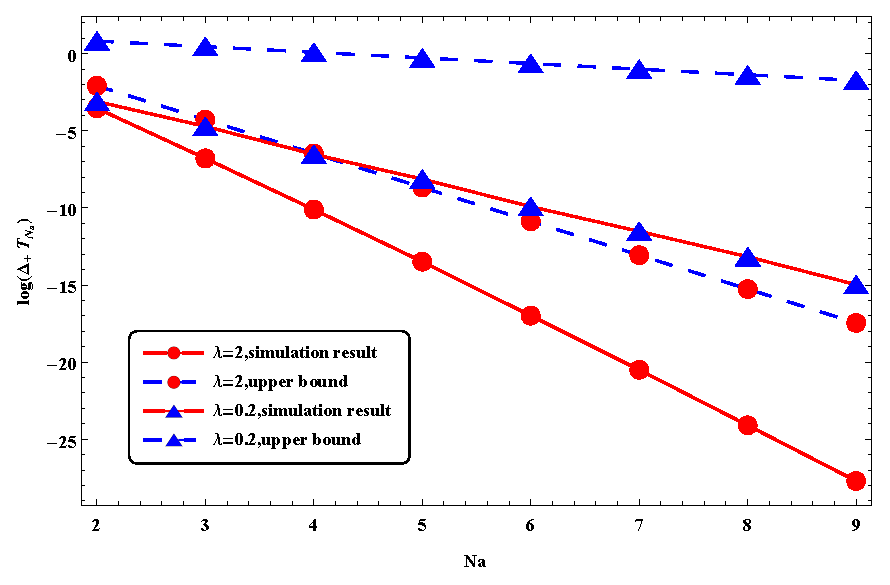
\includegraphics[width=280pt]{decreasing_exponential.eps}
%  \caption{连分式指数收敛性图示}\label{fig:continuous_fraction_exponential}
%\end{figure}
%\end{frame}
%\cfrac{1}{1+\cfrac{z^2}{3-z^2+\cfrac{(3z)^2}{5-3z^2-\cfrac{(5z)^2}{7-5z^2+ \cfrac{(7z)^2}{9-7z^2-\dots}}}}}
%\begin{frame}
%\begin{align*}
%\bm{K}_1&=\lambda \bm{I}_2+(1-\bm{u}_1^{\textrm{T}}\bm{K}_2^{-1}\bm{u}_1)\bm{u}_1\bm{u}_1^{\textrm{T}}\\
%\bm{K}_2&=\lambda \bm{I}_2+\bm{u}_1\bm{u}_1^{\textrm{T}}+(1-\bm{u}_2^{\textrm{T}}\bm{K}_3^{-1}\bm{u}_2)\bm{u}_2\bm{u}_2^{\textrm{T}}\\
%\dots & =\dots\\
%\bm{K}_n&=\lambda \bm{I}+\bm{u}_{n-1}\bm{u}_{n-1}
%\end{align*}
%$\bm{K}_1$的两个特征值是什么?
%
%一个特征值是$\lambda$,
%另一个特征值是$\tilde{\lambda}_1$
%设$\bm{u}_i$和$\bm{u}_{i+1}$的夹角是$\theta_i$,$\tilde{\lambda}_i$是$\bm{K}_i-\bm{u}_{i-1}\bm{u}_{i-1}^{\textrm{T}}$的不等于$\lambda$的那个特征值,$\bm{u}_{0}=\bm{0}$。
%\[
%\tilde{\lambda}_1=\lambda+\frac{1}{1+\frac{\sin^2\theta_1}{\lambda}+\frac{\cos^2\theta_1}{\tilde{\lambda}_2}}
%\]

%\[
%\arctan z
%=\cfrac{1}{1+\cfrac{z^2}{3-z^2+\cfrac{(3z)^2}{5-3z^2+\cfrac{(5z)^2}{7-5z^2+ \cfrac{(7z)^2}{9-7z^2-\dots}}}}},|z|<1
%\]
%上式令$z=1$得到无理数$\pi$的一种连分式展开
%\end{frame}
%\begin{frame}
%\[
%\sum_{x_1=1}^5\sum_{x_2=x_1}^5\dots\sum_{x_{12}=x_{11}}^5 1
%\]
%0<=x1<=x2<=...<=x12<=5,设r1=x1,r2=x2-x1,...r12=x12-x11,r13=5-x12,则
%\[
%r1+r2+\dots+r13=5,0\leq ri
%\]
%推出
%\[
%(r1+1)+(r2+1)+\dots+(r13+1)=17=1+1+\dots+1,1\leq ri+1
%\]
%从等式右边16个加号里取12个加号...
%\end{frame}
%

\section{小结}
\begin{frame}{小结}
在单节点时间协作的定位网络中,
\begin{itemize}
\item 直接法可以得到直线情形下费舍尔信息矩阵的全部特征值,获得时间协作数量趋于无穷大时的定位误差下界。
\item 连分式法可以得到时间终点位置处的信息椭圆,以及增加协作链路后信息量的衰减情况。
\end{itemize}
     \begin{figure}
          \centering
          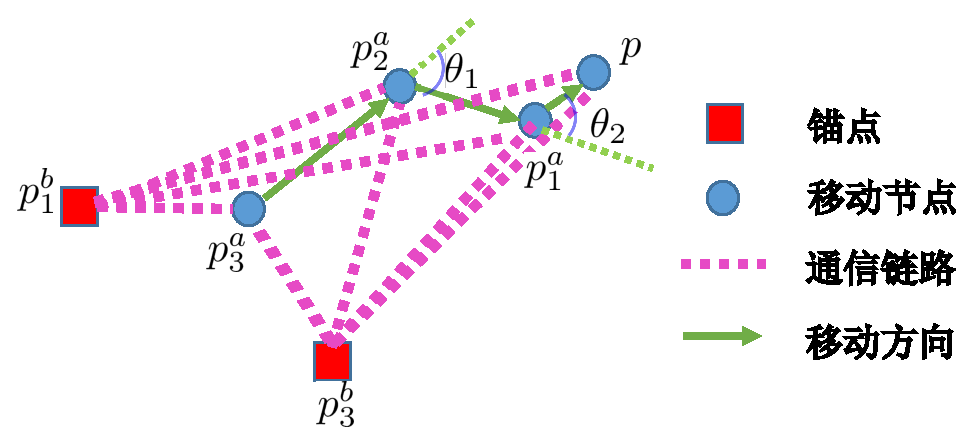
\includegraphics[height=4cm]{cooperative_single_temporal.eps}
          \caption*{时间协作定位图示}
     \end{figure}
\end{frame}
\appendix
\begin{frame}[noframenumbering]
直接求解该问题需要如下两个引理:
\begin{lemma}\label{lemma:change}
设L是$m\times n$的矩阵,$a,\epsilon > 0$则
\begin{equation*}
|a\bm{I}_m+\epsilon \bm{L}\bm{L}^{\textrm{T}}|=a^m|\bm{I}_n+\frac{\epsilon}{a} \bm{L}^{\textrm{T}}\bm{L}|
\end{equation*}
\end{lemma}
\begin{proof}
不妨设$a=\epsilon=1$,
考虑到
\[
\left(\begin{array}{cc}
\bm{I}_n+\bm{L}^{\textrm{T}}\bm{L}&\bm{0}\\
\bm{L}&\bm{I}_m\\
\end{array}\right)\sim\left(\begin{array}{cc}
\bm{I}_n&-\bm{L}^{\textrm{T}}\\
\bm{L}&\bm{I}_m\\
\end{array}\right)\sim\left(\begin{array}{cc}
\bm{I}_n&-\bm{L}^{\textrm{T}}\\
0&\bm{I}_m+\bm{L}\bm{L}^{\textrm{T}}\\
\end{array}\right)
\]
其中$\sim$表示矩阵相抵,两边取行列式即得$|\bm{I}_m+\bm{L}\bm{L}^{\textrm{T}}|=|\bm{I}_n+\bm{L}^{\textrm{T}}\bm{L}|$。
\end{proof}
\end{frame}
\begin{frame}[noframenumbering]
\begin{lemma}\label{lemma:special}
$\bm{S}_{n-1}$是一个n-1维的方阵,
$\bm{S}=\left(
\begin{array}{cccc}
0&1&\dots&0\\
1&0&\dots&0\\
\vdots&\vdots&\ddots&\vdots\\
0&\dots&1&0\\
\end{array}\right).$
则$\bm{S}_{n-1}$的n-1个特征值为:
$\lambda_j=2\cos(\frac{\pi j}{n}),j=1,2,...,n-1$
\end{lemma}
\begin{proof}
\begin{enumerate}
  \item 用数学归纳法证明$S_n$的特征多项式有递推公式$P_n(\lambda)=\lambda P_{n-1}(\lambda)-P_{n-2}(\lambda)$
  \item $U_n(\lambda)=\frac{1}{\sqrt{1-(\frac{\lambda}{2})^2}}\sin((n+1)\arccos(\frac{\lambda}{2}))$适合上面的递推关系式。
  \item $U_1(\lambda),U_2(\lambda)$是多项式,所以$U_n(\lambda)$是关于$\lambda$的多项式
\end{enumerate}
\end{proof}
\end{frame}
\begin{frame}[noframenumbering]{直接法}
不妨设节点沿x轴运动,费舍尔信息矩阵$I(\bm{P})$化简为:
\begin{equation*}
I(\bm{P})=a\bm{I}+b \left(
\begin{array}{ccccc}
\bm{e}_1\bm{e}_1^{\textrm{T}}&-\bm{e}_1\bm{e}_1^{\textrm{T}}&\dots&&0\\
-\bm{e}_1\bm{e}_1^{\textrm{T}}&2\bm{e}_1\bm{e}_1^{\textrm{T}}&-\bm{e}_1\bm{e}_1^{\textrm{T}}&\dots&0\\
\vdots &\vdots&&\ddots &\vdots\\
0&&\dots&-\bm{e}_1\bm{e}_1^{\textrm{T}}&\bm{e}_1\bm{e}_1^{\textrm{T}}\\
\end{array}
\right)
\end{equation*}
其中$\bm{e}_1=\binom{1}{0}$
\end{frame}
\begin{frame}[noframenumbering]
$I(\bm{P})=a\bm{I}+b \bm{L}\bm{L}^{\textrm{T}}$,其中\\

\bigskip
$\bm{e}_1=\binom{1}{0}$且
$\bm{L}=\left(\begin{array}{ccccc}
\bm{e}_1&0&\dots&&0\\
-\bm{e}_1&\bm{e}_1&0&\dots&0\\
\vdots &\vdots&&\ddots &\vdots\\
0&&\dots&-\bm{e}_1&0\\
\end{array}
\right)_{2n\times n}$
\bigskip

$\bm{L}$的最后一列全为零。
\end{frame}
\begin{frame}[noframenumbering]{$I(\bm{P})=a\bm{I}+b \bm{L}\bm{L}^{\textrm{T}}$}
$\bm{I}(\bm{P})$的特征多项式为$|(\lambda-a)\bm{I}-b\bm{L}\bm{L}^{\textrm{T}}|$
\pause

根据引理(\ref{lemma:change}),$|(\lambda-a)\bm{I}-bLL^{\textrm{T}}|=(\lambda-a)^{2n}|\bm{I}_n-\frac{b}{\lambda-a}L^{\textrm{T}}L|$
\[L^{\textrm{T}}L=\left(
\begin{array}{ccccc}
2&-1&\dots&&0\\
-1&2&-1&\dots&0\\
0&-1&2&\dots&0\\
\vdots &\vdots&&\ddots &\vdots\\
0&\dots&&0&0\\
\end{array}
\right).
\]
\pause
设$\bm{K}_{n-1}$为$L^{\textrm{T}}L$第n-1阶主子式,则
$|(\lambda-a)\bm{I}-bLL^{\textrm{T}}|=(\lambda-a)^{n+1}|(\lambda-a)\bm{I}_{n-1}-b\bm{K}_{n-1}|$
\end{frame}
\begin{frame}[noframenumbering]
$\bm{K}_{n-1}=2\bm{I}_{n-1}-\bm{S}$,由引理(\ref{lemma:special})可求出$\bm{K}_{n-1}$的全部特征值。
\pause
\[
f(n):=\frac{\tr(\bm{I}(\bm{P})^{-1})}{n}=\frac{1}{n}\left(\frac{n+1}{a}+\sum_{j=1}^{n-1}\frac{1}{a+2b(1-\cos(\frac{\pi j}{n}))}\right)
\]
当$n\to \infty$,根据Riemann积分的定义:
\[
\lim_{n\rightarrow \infty}f(n)=\frac{1}{a}+\int_0^1 \frac{1}{a+2b(1-\cos(\pi x))}dx
\]
化为复积分由留数定理可得
\[
\lim_{n\rightarrow \infty}f(n)=\frac{1}{a}+\frac{1}{\sqrt{a^2+4ab}}.
\]
\end{frame}
\begin{frame}[noframenumbering]{连分式法推导过程}
提取公因子后,下面用连分式法研究$\bm{I}(\bm{P})=\lambda \bm{I}+\bm{J}$的结构。
\pause
$t_{i}$时刻的位置信息椭圆为
\[
\bm{e}_{i}^{\textrm{T}}(\bm{I}(\bm{P}))^{-1}\bm{e}_{i}
\]
其中
\begin{equation*}
\bm{e}_i=(\bm{0},\dots,\underbrace{\bm{I}_2}_{i\text{-th item}},\dots,\bm{0})^{\textrm{T}}.
\end{equation*}
\end{frame}
\begin{frame}[noframenumbering]
$\bm{I}(\bm{P})$可以简写为:
\begin{equation*}
\bm{I}(\bm{P})=\begin{pmatrix}
                 \bm{B}_1 & \bm{A}_2 & \bm{0} & \dots & \bm{0} \\
                 \bm{A}_2 & \bm{B}_2 & \bm{A}_3 & \dots & \bm{0} \\
                 \vdots & \vdots & \vdots & \ddots & \vdots \\
                 \bm{0} & \dots & \bm{0} & \bm{A}_{N_a} & \bm{B}_{N_a}
               \end{pmatrix}.
\end{equation*}

$\bm{I}(\bm{P})$可以做LU分解如下:
\pause
\begin{equation*}\label{eq:LU}
  \bm{I}(\bm{P})=\begin{pmatrix}
                 \bm{I}_2 & \bm{0} & \bm{0} & \dots & \bm{0} \\
                 \bm{L}_2 & \bm{I}_2 & \bm{0} & \dots & \bm{0} \\
                 \vdots & \vdots & \vdots & \ddots & \vdots \\
                 \bm{0} & \dots & \bm{0} & \bm{L}_{N_a} & \bm{I}_{2}
               \end{pmatrix}\begin{pmatrix}
                 \bm{U}_1 & \bm{A}_2 & \bm{0} & \dots & \bm{0} \\
                 \bm{0} & \bm{U}_2 & \bm{A}_3 & \dots & \bm{0} \\
                 \vdots & \vdots & \vdots & \ddots & \vdots \\
                 \bm{0} & \dots & \bm{0} & \bm{0} & \bm{U}_{N_a}
               \end{pmatrix}.
\end{equation*}
\end{frame}
\begin{frame}[noframenumbering]
$\bm{U}_i$满足如下递推关系:
\begin{equation*}
\begin{cases}
  \bm{U}_1 &= \bm{B}_1 \\
  \bm{U}_i &= \bm{B}_i-\bm{A}_i\bm{U}_{i-1}^{-1}\bm{A}_i,i\geq 2.
\end{cases}
\end{equation*}

其中
\begin{equation*}
\begin{cases}
  \bm{A}_i &= -\bm{u}_i\bm{u}_i^{\textrm{T}} \\
  \bm{B}_i &=\lambda\bm{I}_2+\bm{u}_{i-1}\bm{u}_{i-1}^{\textrm{T}}+\bm{u}_i\bm{u}_i^{\textrm{T}}, 2 \leq i \leq N_a-1.
\end{cases}
\end{equation*}
\end{frame}
\begin{frame}[noframenumbering]
\begin{equation*}\label{eq:LU}
  \bm{I}(\bm{P})=\begin{pmatrix}
                 \bm{I}_2 & \bm{0} & \bm{0} & \dots & \bm{0} \\
                 \bm{L}_2 & \bm{I}_2 & \bm{0} & \dots & \bm{0} \\
                 \vdots & \vdots & \vdots & \ddots & \vdots \\
                 \bm{0} & \dots & \bm{0} & \bm{L}_{N_a} & \bm{I}_{2}
               \end{pmatrix}\begin{pmatrix}
                 \bm{U}_1 & \bm{A}_2 & \bm{0} & \dots & \bm{0} \\
                 \bm{0} & \bm{U}_2 & \bm{A}_3 & \dots & \bm{0} \\
                 \vdots & \vdots & \vdots & \ddots & \vdots \\
                 \bm{0} & \dots & \bm{0} & \bm{0} & \bm{U}_{N_a}
               \end{pmatrix}.
\end{equation*}

从上式可以求出
\begin{equation*}\label{eq:thomas_final}
\bm{e}_{N_a}^{\textrm{T}}(\bm{I}(\bm{P}))^{-1}\bm{e}_{N_a}=U_{N_a}^{-1}.
\end{equation*}
\pause

关于$U_{N_a}$的结构我们有结论,它的一个特征值是$\lambda$,另一个特征值可以用连分式表示出来。
\end{frame}
\begin{frame}[noframenumbering]
设$\bm{u}_i=(\cos\theta_i,\sin\theta_i)^{\textrm{T}}$
\begin{equation*}
\begin{split}
T_{i-1} =& \lambda + \frac{1}{1+\frac{\sin^2\theta_i}{\lambda}+\frac{\cos^2\theta_i}{T_i}},2\leq i\leq N_a-1\\
T_{N_a-1}  =& \lambda+\frac{1}{1+1/\lambda}
\end{split}
\end{equation*}

$T_1$就是$U_{N_a}$的另一个特征值。
\end{frame}
\begin{frame}[noframenumbering]{连分式与Pad\'e逼近}
可以用归纳法得到
\[
[\lambda,1,\underbrace{\lambda,1}_{\text{$n$ item}}]=\frac{P_{n+1}(\lambda)}{Q_n(\lambda)}
\]
其中$P_{n+1}(\lambda),Q_n(\lambda)$是关于$\lambda$的n+1和n次多项式。
\end{frame}
\begin{frame}[noframenumbering]
有理分式逼近(Pad\'{e}逼近)理论指出对于光滑函数$f(x)$,可构造有理分式:
\[
R_{n+m}(x)=\frac{P_n(x)}{Q_m(x)}
\]
来逼近$f(x)$,使得$R_{n+m}(x)$与$f(x)$在$x=0$处直到$n+m$次导数相等。
\pause


Taylor级数是$m=0$的情形
\pause

函数的有限连分式展开在某些情况下是$|n-m|=1$的情形
\begin{flushright}
\hspace{ \stretch{1} }\fbox{\parbox[b][5em][t]{0.4\textwidth}{Pad\'{e} approximation and continued fractions, Applied Numerical Mathematics, 2010}}
\end{flushright}
\end{frame}
\begin{frame}[noframenumbering]
下面我们考虑$m+n$相等时不同的展开方式对$f(\lambda)=\frac{\lambda+\sqrt{4\lambda+\lambda^2}}{2}$逼近的效果情况,
\pause

由于$f(\lambda)$在$\lambda=0$处有奇性(一阶导数不存在),我们考虑其在复平面关于$\infty$的Taylor展开式,通过令$x=1/\lambda$不难得到
\begin{align}\notag
f(\lambda)=&\frac{2}{\sqrt{1+4x}-1}\\
=&\frac{1}{x-x^2+2x^3-5x^4+14x^5+\dots}
\end{align}

由于$\sqrt{1+4x}$收敛域为$|4x|<1$可得$|\lambda|>4$,可见Taylor展开对$\lambda$的取值有限制。
\end{frame}
\begin{frame}[noframenumbering]
\begin{figure}
\centering
\caption*{取n+m=5对$f(\lambda)$的有理逼近图示}
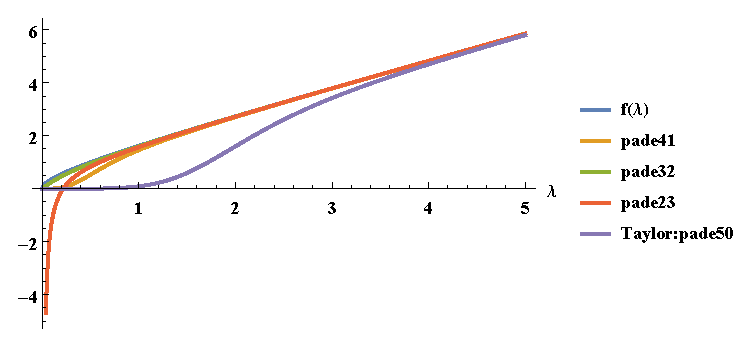
\includegraphics[width=300pt]{pade.eps}
\end{figure}
\begin{itemize}
  \item Taylor展开逼近在$\lambda<4$时偏离较大
  \item pade41收敛域大于Taylor展开,但在$\lambda$较小处仍然不收敛
  \item 连分式对应的pade32对于$\lambda>0$逐点收敛到$f(\lambda)$
\end{itemize}
\end{frame}

%\subsection{正方形网络和正六边形网络}
%\begin{frame}[noframenumbering]
%在正方形网络中,由于正交性,定位效果并不理想。
%  \begin{columns}[T] % contents are top vertically aligned
%     \begin{column}[T]{6cm}
%     右图中$\bm{p}_3$的位置信息要想被$\bm{p}_1$利用提高定位精度,是通过改善$\bm{p}_2$的定位精度间接实现的。
%     \pause
%但是$\bm{p}_3$对$\bm{p}_2$位置精度的贡献的方向恰好与$\bm{p}_2$对$\bm{p}_1$位置精度的贡献的方向垂直,因此$\bm{p}_3$对$\bm{p}_1$定位精度的提高没有贡献。
%     \end{column}
%     \begin{column}[T]{5cm} % alternative top-align that's better for graphics
%          \includegraphics[height=4cm]{orthogonal.eps}
%     \end{column}
%     \end{columns}
%\end{frame}
%\begin{frame}[noframenumbering]
%在正六边形网络中,类似线性网络中的直接法,
%通过采用节点分层技术可以得到网络规模趋向于无穷大时的节点平均定位误差下界为
%  \begin{equation}
%  \lambda+\frac{3}{2}-\cfrac{3/2}{\lambda+\frac{3}{2}-\cfrac{1/2}{\lambda+3/2-\dots}}=\sqrt{\lambda^2+3\lambda+\frac{1}{4}}-\frac{1}{\lambda+\frac{3}{2}+\sqrt{\lambda^2+3\lambda+\frac{1}{4}}}.
%  \end{equation}
%\end{frame}
%\begin{frame}[noframenumbering]
%  在数学方法方面,本文主要的成果如下:
%  \begin{itemize}
%  \item
%    使用复数表示法推导得出非协作定位场景下费舍尔信息矩阵的特征值和特征向量的表达式。
%  \item
%    推导得出秩一矩阵的克罗内克积对N维对称正定矩阵扰动后行列式的表达式。
%  \item
%    推导得出二维场景下特殊完全图的邻接矩阵所有特征值,其中使用瑞利商给出了最大 特征值的表达式。
%  \item 推导得出二维场景下特殊度为2的图的邻接矩阵的所有特征值;当网络规模趋向无穷大时,求出了所有特征值的倒数和的平均值的极限。
%  \item 使用连分式推导得出形如$\lambda \bm{I}+\bm{J}$的对称正定矩阵$\bm{A}$确定的$\bm{A}^{-1}_{1\times2,1\times2}$的两个特征值;分析得出了决定特征值的连分式的序列指数收敛的特性,并做出适当的推广。
%  \end{itemize}
%
%\end{frame}
%\begin{frame}[noframenumbering]
% \frametitle{参考文献}
% \tiny
% \begin{itemize}
%   \item Kegen Yu I S, Guo Y J. Ground-Based Wireless Positioning. John Wiley and Sons, Ltd,2009
%   \item L J, S L, G V. Development and experimental validation of an adaptive extended kalman filter for the localization of mobile robots. IEEE Transactions, 1999, 15(2):219–229
%   \item Shen Y, Win M Z, Wymeersch H. Fundamental limits of wideband localization—part
%i: A general framework. IEEE TRANSACTIONS ON INFORMATION THEORY, 2010,
%56(10):4956–4980
%   \item 杨思怡. 协作定位网络的信息耦合机理 [D]. 北京: 清华大学, 2016
%   \item 姚慕生. 高等代数学. 上海: 复旦大学出版社, 2003
%   \item MazuelasS,ShenY,WinMZ. Spatio-temporalinformationcouplingincooperativenetwork
%navigation. Globecom Communication Theory Symposium, 2012. 2403–2407
%   \item 关治, 陆金甫. 数值分析基础. 北京: 高等教育出版社, 2010: 52–56
%   \item Hammond W F. Continued fractions and the euclidean algorithm. Lecture notes, University
%at Albany, 1997
% \end{itemize}
%\end{frame}

\end{document}


